\section{Habanero Java Overview}
The Habanero Java Programming model was built as an extension to the Java-based definition of the X10 language. The Habanero Java Library (HJ-lib) is a Java 8 library implementation of the Habanero Java Programming model. It includes a set of powerful parallel programming constructs that can be used to create programs that are inherently safe. HJ-Lib puts particular emphasis on the usability and safety of parallel programming constructs. For example, no HJ program written using async, finish, isolated and phaser constructs can create a logical deadlock cycle. HJ-Lib creates standard Java class files that can be run on any Java 8 JVM. 

\subsection{\textbf{HJ constructs}}
HJ consists of a wide range of constructs for parallel programming.
\begin{itemize}
\item \textbf{Task Spawn and Join:} Async and finish constructs are used to create and join tasks created by a parent process. The statement async(() $ \rightarrow \langle$stmt$\rangle$) creates a new task that can logically execute in parallel with its parent task. The Finish method is used to represent join in Habanero Java. The task executing finish(() $ \rightarrow \langle$stmt$\rangle$) has to wait for all the tasks running inside stmt to finish before it can move on.
\item \textbf{Loop Parallelism:} The forall and forasync constructs in HJ are used for loop parallelism. An implicit finish is included at the end of forall iterations whereas forasync iterations do not have an implicit finish. 
\item \textbf{Coordination Constructs:} There are often dependencies among parallel tasks. To coordinate the execution of the parallel tasks, HJ provides some constructs such as isolated, futures, data-driven futures and phasers.
\begin{itemize}
\item \textbf{Isolated:} Most of the concurrently running processes have the need to synchronize the access to the shared variables. The isolated statements allow only one process at a time to access referenced shared variables. Isolated statements create performance bottlenecks in moderate to high contention systems. HJ also provides object-based isolation which provides better performance.
\item \textbf{Futures:} HJ supports returning values from a newly created child task to the parent task with the help of futures. The statement HjFuture$\langle$T$\rangle$ f = future $\langle$T$\rangle$ (() $ \rightarrow \langle$expr$\rangle$) creates a new child task which executes expr and the result of this execution can be obtained by the parent task by calling f.get() method.
\item \textbf{Data-driven futures:} DDFs are an extension to futures. Any async can register on a DDF as a consumer causing the execution of the async to be delayed until a value becomes available in the DDF. The exact syntax for an async waiting on a DDF is as follows: asyncAwait(ddf1, ... , ddfN, () $\rightarrow$ stmt). An async waiting on a chain of DDFs can only begin executing after a put() has been invoked on all the DDFs.
\item \textbf{Phasers} - Phasers help in point-to-point synchronization. Each task has the option of registering with a phaser in signal-only/wait-only mode for producer/consumer synchronization or signal-wait mode for barrier synchronization. A task may be registered on multiple phasers, and a phaser may have multiple tasks registered on it. Phasers ensure deadlock freedom when programmers use only the next statements in their programs. In programs where tasks are involved with multiple point-to-point coordination, explicit use of doWait() and doSignal() on multiple phasers might be required.  
\end{itemize}
\end{itemize}

\subsection{\textbf{HJ Sample Program}}
Fig. 1 shows a sample program written in HJ. In this example, the main process starts two new processes running in parallel with the process. The main process has to stop its execution at the end of finish block and wait for the child processes to complete their execution before the main process can proceed further. Both the newly spawned processes have a co-ordination construct 'isolated' that creates nodes s and s' in the computation graph. There is a serialization edge between s and s' that shows the ordering of the events in this execution. This results in a computation graph shown in Fig. 2. 

\begin{figure}
  \begin{center}
    \begin{lstlisting}
public class Example1{
    static int x = 0;
    public static void main(String[] args) {
	launchHabaneroApp(() -> {
	    finish(() -> {
		async(() -> { //Thread1
		    isolated(() -> {
			x++; 	//Isolated block s
		    });			
		});
		async(() -> { //Thread2
		    isolated(() -> {
			x++; 	//Isolated block s'
		    });			
		});
	    });
	 });
    }
}
\end{lstlisting}
  \end{center}
  \caption{Sample HJ Program}
  \label{fig:hj-async-finish-isolated}
\end{figure}

\begin{figure}[t]
  \centering
    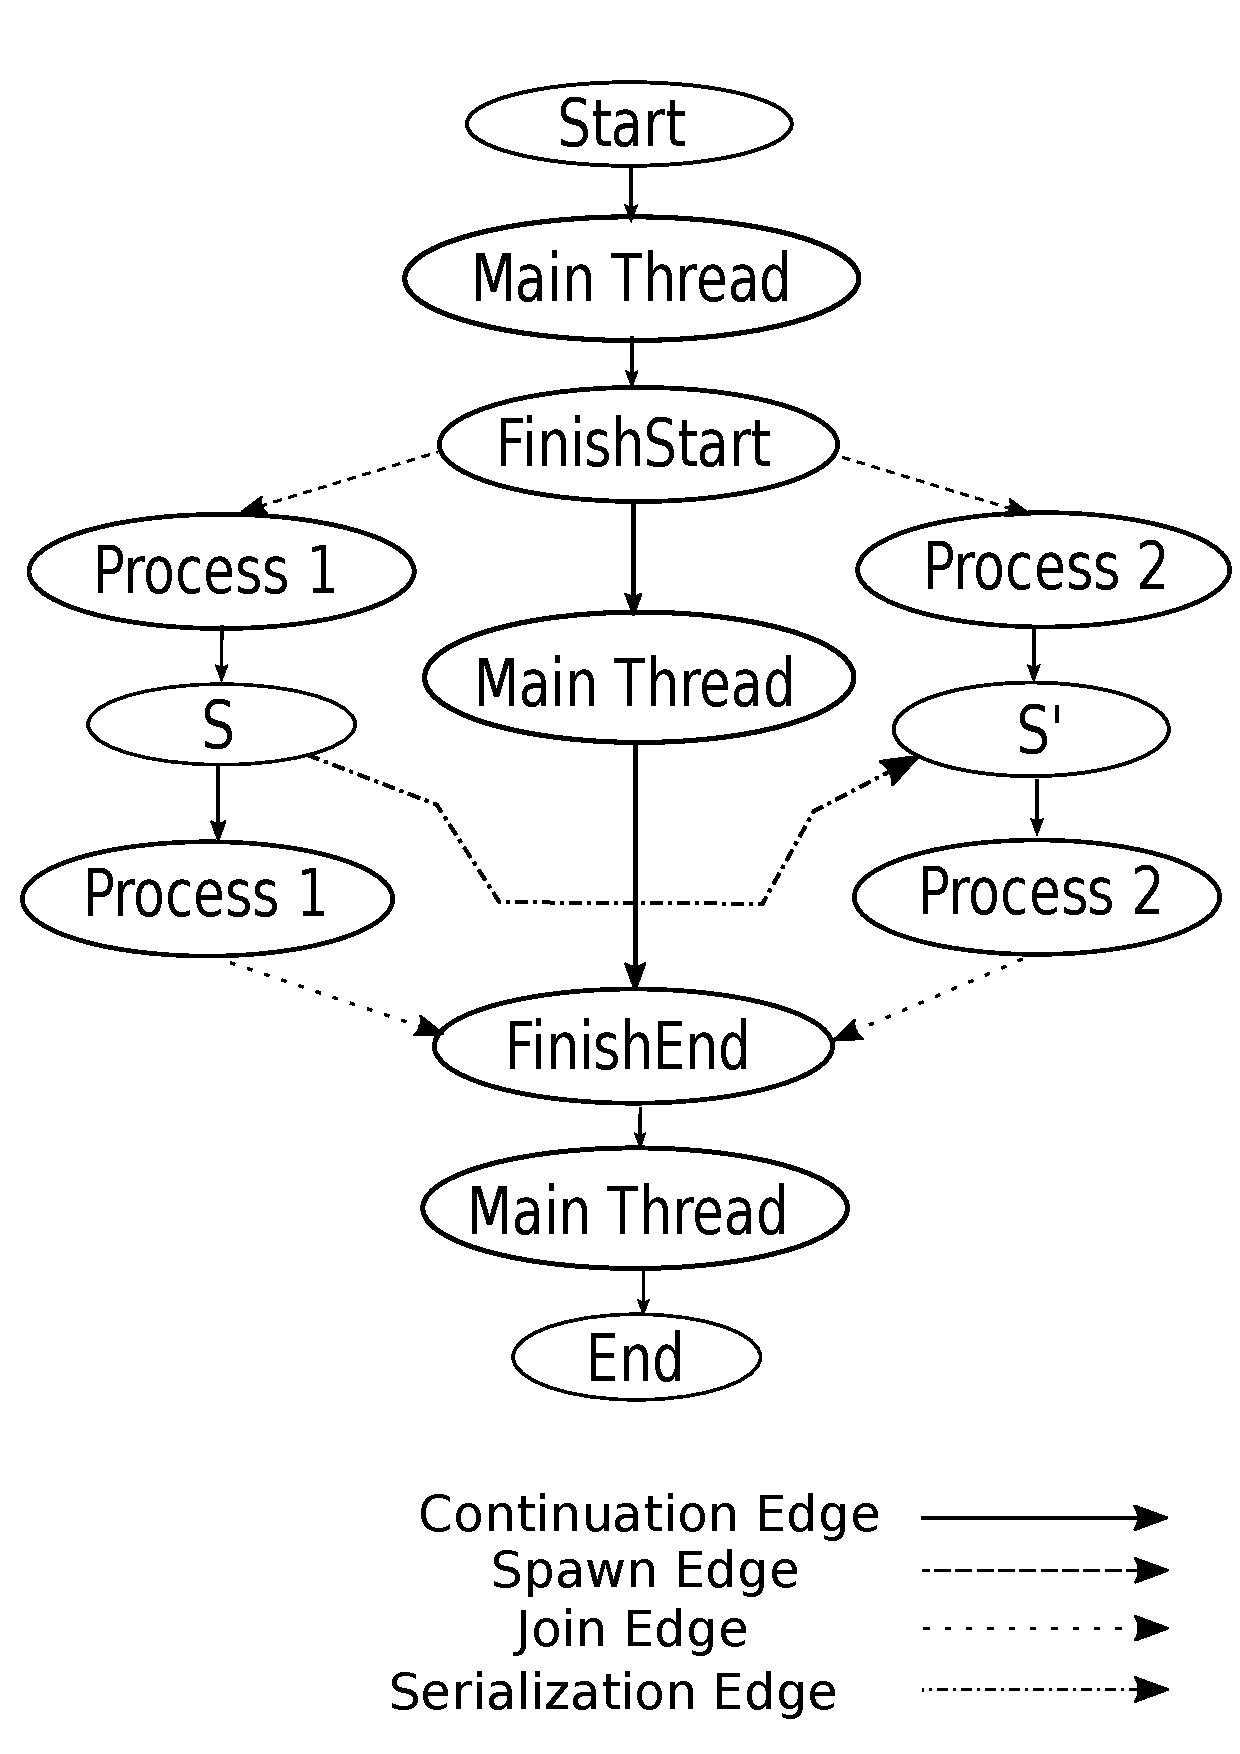
\includegraphics[width=0.4\textwidth]{../figs/drawing.pdf}
    \caption{Computation Graph of the Sample program}
\end{figure}
